\documentclass[11pt,letterpaper]{article}
\usepackage[margin=1.25in]{geometry}
\usepackage{palatino}
\usepackage{microtype}
\usepackage{parskip}
\usepackage{xcolor}
\usepackage{titlesec}
\usepackage{fancyhdr}
\usepackage{enumitem}
\usepackage{booktabs}
\usepackage{longtable}
\usepackage{amsmath}
\usepackage{amssymb}
\usepackage{graphicx}
\usepackage{hyperref}
\usepackage{tikz}
\usetikzlibrary{shapes.geometric, arrows, positioning}

% Define colors
\definecolor{accentblue}{RGB}{0,70,127}
\definecolor{darkgray}{RGB}{64,64,64}
\definecolor{lightgray}{RGB}{245,245,245}
\definecolor{alertred}{RGB}{180,0,0}
\definecolor{successgreen}{RGB}{0,120,60}

% Section formatting
\titleformat{\section}
  {\Large\bfseries\color{accentblue}}
  {\thesection}
  {1em}
  {}

\titleformat{\subsection}
  {\large\bfseries\color{darkgray}}
  {\thesubsection}
  {1em}
  {}

\titleformat{\subsubsection}
  {\normalsize\bfseries\color{darkgray}}
  {\thesubsubsection}
  {1em}
  {}

% Header/footer
\pagestyle{fancy}
\fancyhf{}
\renewcommand{\headrulewidth}{0.4pt}
\fancyhead[L]{\small\color{darkgray} Marketing Measurement Methodology}
\fancyhead[R]{\small\color{darkgray} Technical Design Document}
\fancyfoot[C]{\thepage}

% Hyperref setup
\hypersetup{
    colorlinks=true,
    linkcolor=accentblue,
    urlcolor=accentblue
}

% Custom environments
\newenvironment{principle}[1]{%
    \begin{quote}
    \textbf{\color{accentblue}Principle: #1}\\[0.5em]
    \itshape
}{%
    \end{quote}
}

\newenvironment{checkpoint}{%
    \begin{quote}
    \textbf{\color{successgreen}Quality Gate}\\[0.3em]
}{%
    \end{quote}
}

\newenvironment{antipattern}{%
    \begin{quote}
    \textbf{\color{alertred}Anti-Pattern}\\[0.3em]
}{%
    \end{quote}
}

\begin{document}

\begin{center}
{\LARGE\bfseries\color{accentblue} Marketing Measurement Methodology}\\[0.5em]
{\large Technical Design Document}\\[1em]
{\normalsize A Rigorous Workflow from Business Question to Validated Insight}\\[1.5em]
{\small VERSION 1.0 --- \today}\\[0.5em]
{\small INTERNAL REFERENCE DOCUMENT}
\end{center}

\vspace{1em}

\tableofcontents
\newpage

%==============================================================================
\section{Executive Overview}
%==============================================================================

This document specifies a complete methodology for marketing measurement engagements, from initial client conversation through final deliverables. The workflow is designed to produce credible, validated, and actionable insights while avoiding the methodological pitfalls that undermine traditional approaches.

\subsection{Design Principles}

The methodology is built on five core principles:

\begin{enumerate}[leftmargin=1.5em, itemsep=0.5em]
    \item \textbf{Question-first scoping.} Projects are defined by the business decisions they inform, not by deliverables or model counts. The question determines the method, not the reverse.
    
    \item \textbf{Pre-specification.} Key analytical choices are documented before seeing results. This eliminates specification shopping and makes the analysis auditable.
    
    \item \textbf{Uncertainty quantification.} Every estimate includes honest uncertainty bounds. When we don't know, we say so---and recommend how to reduce uncertainty.
    
    \item \textbf{Validation integration.} Where feasible, model predictions are tested against experimental results. Validation creates accountability and improves calibration over time.
    
    \item \textbf{Transparent reporting.} Deliverables distinguish between robust and fragile findings, acknowledge limitations, and provide decision-makers with the information needed to act appropriately.
\end{enumerate}

\subsection{Workflow Phases}

The methodology consists of six phases:

\begin{center}
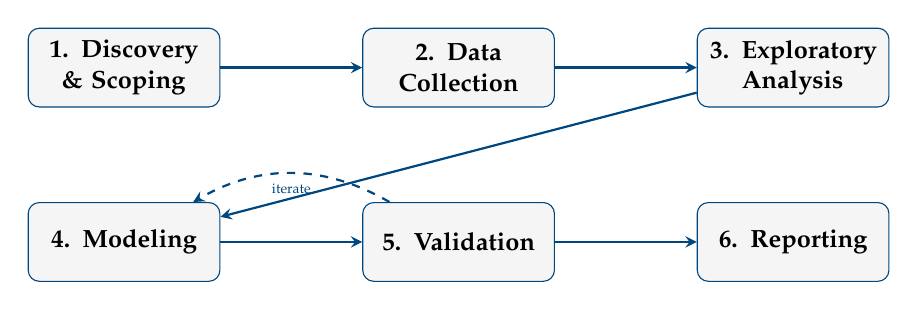
\begin{tikzpicture}[node distance=1.8cm, auto,
    phase/.style={rectangle, rounded corners, draw=accentblue, fill=lightgray, 
                  text width=2.2cm, minimum height=1cm, align=center, font=\small\bfseries},
    arrow/.style={->, >=stealth, thick, accentblue}]
    
    \node[phase] (discover) {1. Discovery \& Scoping};
    \node[phase, right=of discover] (data) {2. Data Collection};
    \node[phase, right=of data] (eda) {3. Exploratory Analysis};
    \node[phase, below=1.2cm of discover] (model) {4. Modeling};
    \node[phase, right=of model] (validate) {5. Validation};
    \node[phase, right=of validate] (report) {6. Reporting};
    
    \draw[arrow] (discover) -- (data);
    \draw[arrow] (data) -- (eda);
    \draw[arrow] (eda) -- (model);
    \draw[arrow] (model) -- (validate);
    \draw[arrow] (validate) -- (report);
    \draw[arrow, dashed] (validate) to[bend right=30] node[below, font=\tiny] {iterate} (model);
\end{tikzpicture}
\end{center}

Each phase has defined inputs, outputs, quality gates, and decision points. The remainder of this document specifies each phase in detail.

\newpage
%==============================================================================
\section{Phase 1: Discovery and Scoping}
%==============================================================================

\begin{principle}{Start with the decision, not the data.}
The purpose of measurement is to inform decisions. Before discussing data or methods, understand what decisions the analysis must support, what precision those decisions require, and what actions will follow from different findings.
\end{principle}

\subsection{Objectives}

\begin{itemize}[leftmargin=1.5em, itemsep=0.3em]
    \item Identify the specific business decisions the engagement must inform
    \item Assess data availability and quality constraints
    \item Determine appropriate methodology given question, data, and timeline
    \item Establish success criteria and validation approach
    \item Document scope, assumptions, and limitations in a signed charter
\end{itemize}

\subsection{Discovery Meeting Structure}

The initial discovery session should address the following areas:

\subsubsection{Business Context (30--45 minutes)}

\begin{itemize}[leftmargin=1.5em, itemsep=0.3em]
    \item What decisions will this analysis inform?
    \item When must decisions be made? (Timeline constraints)
    \item What is the cost of a wrong decision? (Stakes calibration)
    \item What actions are available? (Decision space)
    \item Who are the decision-makers and what is their analytical sophistication?
    \item What prior beliefs exist about channel effectiveness?
    \item Have previous measurement efforts been conducted? What were the results?
\end{itemize}

\subsubsection{Measurement History (15--20 minutes)}

\begin{itemize}[leftmargin=1.5em, itemsep=0.3em]
    \item What measurement approaches have been used previously?
    \item What worked well? What created problems?
    \item Were results ever validated against experiments or holdouts?
    \item What caused year-over-year instability in past estimates (if any)?
    \item Are there channels where stakeholders have strong priors?
\end{itemize}

\subsubsection{Data Landscape (30--45 minutes)}

\begin{itemize}[leftmargin=1.5em, itemsep=0.3em]
    \item What outcome data is available? (Sales, conversions, brand metrics)
    \item At what granularity? (National, regional, DMA, store, individual)
    \item What is the time resolution? (Daily, weekly, monthly)
    \item How far back does reliable data extend?
    \item What media data is available? (Spend, impressions, GRPs)
    \item Is media data at the same granularity as outcome data?
    \item What control variables are available? (Pricing, distribution, competitive, economic, weather)
    \item Are there known data quality issues?
\end{itemize}

\subsubsection{Experimental Feasibility (15--20 minutes)}

\begin{itemize}[leftmargin=1.5em, itemsep=0.3em]
    \item Is geographic or temporal variation in media feasible?
    \item Have geo experiments or holdout tests been run?
    \item Are platform-run lift studies available for calibration?
    \item What is the appetite for designing validation experiments?
\end{itemize}

\subsection{Question Classification Framework}

Different questions require different methods. Classify the primary question:

\begin{longtable}{p{4cm}p{4cm}p{5cm}}
\toprule
\textbf{Question Type} & \textbf{Example} & \textbf{Appropriate Methods} \\
\midrule
\endhead
Budget allocation & ``How should we distribute \$50M across channels?'' & MMM with uncertainty-aware optimization, sensitivity analysis \\
\addlinespace
Channel effectiveness & ``What is the ROI of our TV investment?'' & MMM with experimental calibration, geo tests \\
\addlinespace
Incrementality & ``How many conversions did this campaign cause?'' & Geo experiments, matched market tests, synthetic control \\
\addlinespace
Saturation \& diminishing returns & ``Are we overspending on search?'' & MMM with flexible saturation curves, marginal ROI analysis \\
\addlinespace
Brand vs. performance & ``How does brand advertising affect long-term sales?'' & Dynamic models, brand health integration, long-horizon analysis \\
\addlinespace
Attribution & ``Which touchpoints contribute to conversion?'' & Multi-touch attribution (with caveats), path analysis \\
\addlinespace
Forecasting & ``What will happen if we cut spend by 20\%?'' & Causal models with out-of-sample validation \\
\bottomrule
\end{longtable}

\subsection{Methodology Selection Matrix}

Based on question type and data availability, select the primary methodology:

\begin{longtable}{p{3cm}p{3cm}p{3cm}p{4cm}}
\toprule
\textbf{Data Granularity} & \textbf{Media Variation} & \textbf{Experimental Feasibility} & \textbf{Recommended Approach} \\
\midrule
\endhead
National only & National only & Low & Aggregate MMM with wide uncertainty bounds; strong recommendation for geo testing \\
\addlinespace
DMA/Regional & National or regional & Low & Hierarchical MMM with geo random effects \\
\addlinespace
DMA/Regional & Regional variation exists & Medium & Hierarchical MMM + matched market validation \\
\addlinespace
DMA/Regional & Can create variation & High & Geo experiment as primary; MMM for extrapolation \\
\addlinespace
Store/Individual & High granularity & High & Individual-level models; A/B or geo tests for validation \\
\bottomrule
\end{longtable}

\subsection{Scope Document Requirements}

The discovery phase concludes with a signed scope document containing:

\begin{enumerate}[leftmargin=1.5em, itemsep=0.3em]
    \item \textbf{Business question statement:} The specific decisions this analysis will inform, stated in operational terms
    \item \textbf{Success criteria:} What constitutes a successful engagement (not ``positive ROI'' but ``credible ROI estimate with defined uncertainty'')
    \item \textbf{Methodology overview:} Primary and secondary methods to be employed
    \item \textbf{Data requirements:} Specific data needed, responsible parties, delivery timeline
    \item \textbf{Pre-registration summary:} Key analytical choices made before seeing data
    \item \textbf{Validation plan:} How results will be validated (experiments, holdouts, sensitivity analysis)
    \item \textbf{Timeline and milestones:} Phase deliverables and decision points
    \item \textbf{Limitations and assumptions:} Known constraints, caveats, and boundaries of the analysis
    \item \textbf{Out of scope:} Explicit statement of what the engagement will not address
\end{enumerate}

\begin{checkpoint}
Before proceeding to Phase 2, confirm:
\begin{itemize}[leftmargin=1.5em, itemsep=0.2em]
    \item Business question is stated in decision terms, not deliverable terms
    \item Methodology matches question type and data availability
    \item Client understands that results may show uncertainty or null effects
    \item Validation approach is agreed and feasible
    \item Scope document is signed by project sponsor
\end{itemize}
\end{checkpoint}

\newpage
%==============================================================================
\section{Phase 2: Data Collection and Stewardship}
%==============================================================================

\begin{principle}{Data quality determines estimate quality.}
No statistical method can overcome fundamental data problems. Invest in understanding data provenance, identifying quality issues, and documenting limitations before analysis begins.
\end{principle}

\subsection{Objectives}

\begin{itemize}[leftmargin=1.5em, itemsep=0.3em]
    \item Collect all required data per scope document specifications
    \item Validate data quality, completeness, and consistency
    \item Document data provenance, transformations, and known issues
    \item Establish data versioning and change control
    \item Create reproducible data pipeline
\end{itemize}

\subsection{Data Requirements Specification}

\subsubsection{Outcome Data}

\begin{longtable}{p{3cm}p{4cm}p{6cm}}
\toprule
\textbf{Data Element} & \textbf{Ideal Specification} & \textbf{Quality Checks} \\
\midrule
\endhead
Sales/Revenue & Daily or weekly, by geography (DMA minimum) & Check for gaps, outliers, seasonality patterns, negative values \\
\addlinespace
Transaction counts & Daily, by geography and product category & Verify against revenue; check for zero-inflation \\
\addlinespace
Brand metrics & Weekly or monthly, consistent methodology over time & Check for survey methodology changes, sample size stability \\
\addlinespace
Web conversions & Daily, by geography if available & Verify tracking consistency; check for platform changes \\
\bottomrule
\end{longtable}

\subsubsection{Media Data}

\begin{longtable}{p{3cm}p{4cm}p{6cm}}
\toprule
\textbf{Data Element} & \textbf{Ideal Specification} & \textbf{Quality Checks} \\
\midrule
\endhead
TV & Weekly GRPs or impressions by DMA, by daypart if available & Reconcile to spend; check for coverage gaps \\
\addlinespace
Digital display & Daily impressions by geo, by platform & Verify impression definitions are consistent \\
\addlinespace
Paid search & Daily spend and clicks by geo & Check for bid strategy changes affecting spend patterns \\
\addlinespace
Social & Daily impressions/spend by platform, by geo if available & Note organic vs. paid; check for algorithm changes \\
\addlinespace
Radio/Audio & Weekly GRPs by market & Often less granular; document limitations \\
\addlinespace
OOH & Weekly or monthly impressions by market & Verify measurement methodology \\
\bottomrule
\end{longtable}

\subsubsection{Control Variables}

\begin{longtable}{p{3cm}p{4cm}p{6cm}}
\toprule
\textbf{Category} & \textbf{Examples} & \textbf{Notes} \\
\midrule
\endhead
Pricing & Own price, promotional pricing, competitor pricing & Match granularity to outcome data \\
\addlinespace
Distribution & Store count, ACV, out-of-stock rates & Critical for retail; often underweighted \\
\addlinespace
Competitive & Competitor spend (if available), share of voice & Often incomplete; document coverage \\
\addlinespace
Economic & Unemployment, consumer confidence, gas prices & Use consistent geographic matching \\
\addlinespace
Seasonality & Holidays, events, weather & Pre-specify which events to include \\
\addlinespace
COVID/Disruptions & Lockdown indicators, supply chain disruptions & Critical for recent data; structural breaks \\
\bottomrule
\end{longtable}

\subsection{Data Quality Assessment Protocol}

For each data source, complete the following assessment:

\begin{enumerate}[leftmargin=1.5em, itemsep=0.3em]
    \item \textbf{Completeness:} What percentage of expected observations are present? Document gaps.
    \item \textbf{Consistency:} Do values fall within expected ranges? Flag outliers for review.
    \item \textbf{Temporal stability:} Are there structural breaks, methodology changes, or platform updates?
    \item \textbf{Cross-source reconciliation:} Do related data sources agree? (e.g., spend vs. impressions)
    \item \textbf{Granularity match:} Can all data be aligned to a common geographic and temporal grain?
    \item \textbf{Provenance:} Who provided the data? What transformations were applied upstream?
\end{enumerate}

\subsection{Data Documentation Standards}

Create a data dictionary containing:

\begin{itemize}[leftmargin=1.5em, itemsep=0.3em]
    \item Variable name, description, and units
    \item Source system and extraction method
    \item Date range and update frequency
    \item Geographic and temporal granularity
    \item Known issues, caveats, and limitations
    \item Transformations applied (if any)
    \item Quality assessment summary
\end{itemize}

\subsection{Data Versioning and Reproducibility}

\begin{itemize}[leftmargin=1.5em, itemsep=0.3em]
    \item All raw data files stored with version identifiers and extraction timestamps
    \item Data processing scripts version-controlled (Git or equivalent)
    \item Processed datasets include hash checksums for integrity verification
    \item Any manual corrections documented with rationale and approver
    \item Data pipeline is reproducible: running scripts on raw data produces identical processed data
\end{itemize}

\begin{antipattern}
Receiving data in Excel files with undocumented manual adjustments, inconsistent date formats, or values that cannot be reconciled to source systems. If data arrives in this state, pause and invest in cleaning and documentation before proceeding.
\end{antipattern}

\begin{checkpoint}
Before proceeding to Phase 3, confirm:
\begin{itemize}[leftmargin=1.5em, itemsep=0.2em]
    \item All required data received and validated
    \item Data dictionary complete and reviewed
    \item Quality issues documented with mitigation plans
    \item Data pipeline reproducible and version-controlled
    \item Granularity alignment confirmed (all data at common grain)
\end{itemize}
\end{checkpoint}

\newpage
%==============================================================================
\section{Phase 3: Exploratory Data Analysis}
%==============================================================================

\begin{principle}{Explore before you model, but document what you learn.}
EDA informs modeling choices but must not become specification shopping. Document insights from exploration, make modeling decisions based on domain knowledge, and resist the temptation to peek at focal relationships before pre-registration.
\end{principle}

\subsection{Objectives}

\begin{itemize}[leftmargin=1.5em, itemsep=0.3em]
    \item Understand data distributions, patterns, and anomalies
    \item Identify potential confounders, structural breaks, and data quality issues
    \item Inform (but not determine) modeling choices
    \item Complete pre-registration document before examining focal relationships
\end{itemize}

\subsection{Permitted and Restricted Analyses}

\subsubsection{Permitted Before Pre-Registration}

\begin{itemize}[leftmargin=1.5em, itemsep=0.3em]
    \item Univariate distributions of all variables
    \item Time series plots of outcome and media variables
    \item Seasonality and trend decomposition
    \item Missing data patterns and outlier identification
    \item Correlation among control variables (multicollinearity assessment)
    \item Stationarity tests for time series
    \item Geographic variation in outcomes and media
\end{itemize}

\subsubsection{Restricted Until After Pre-Registration}

\begin{itemize}[leftmargin=1.5em, itemsep=0.3em]
    \item Correlations between media variables and outcomes
    \item Regression of outcomes on media (even ``exploratory'')
    \item Any analysis that reveals the relationship between focal predictors and response
    \item Specification comparisons (e.g., ``which adstock fits better'')
\end{itemize}

The purpose of this restriction is to ensure that pre-registered modeling choices are based on domain knowledge and theoretical considerations, not on peeking at what ``works'' in the data.

\subsection{Standard EDA Deliverables}

\subsubsection{Outcome Variable Profile}

\begin{itemize}[leftmargin=1.5em, itemsep=0.3em]
    \item Distribution (histogram, summary statistics, skewness)
    \item Time series plot with trend and seasonality decomposition
    \item Geographic variation (coefficient of variation across DMAs)
    \item Outlier identification and proposed treatment
    \item Structural breaks (COVID, supply chain, competitive events)
\end{itemize}

\subsubsection{Media Variable Profiles}

For each media channel:
\begin{itemize}[leftmargin=1.5em, itemsep=0.3em]
    \item Distribution of spend/impressions
    \item Temporal pattern (flighting, seasonality, trends)
    \item Geographic variation (national vs. regional allocation)
    \item Zero-inflation (percentage of observations with no spend)
    \item Correlation with other media channels (flighting overlap)
\end{itemize}

\subsubsection{Control Variable Assessment}

\begin{itemize}[leftmargin=1.5em, itemsep=0.3em]
    \item Distributions and temporal patterns
    \item Multicollinearity assessment (VIF, condition indices)
    \item Correlation matrix among controls
    \item Identification of potentially redundant variables
\end{itemize}

\subsection{Pre-Registration Document}

Before any analysis of media-outcome relationships, complete and file a pre-registration document specifying:

\begin{enumerate}[leftmargin=1.5em, itemsep=0.3em]
    \item \textbf{Model structure:} Functional form (log-log, linear, mixed), hierarchical structure, likelihood (Gaussian, negative binomial)
    
    \item \textbf{Variable transformations:}
    \begin{itemize}[leftmargin=1.5em, itemsep=0.2em]
        \item Adstock specification: decay rates or half-life ranges (based on industry benchmarks, not data)
        \item Saturation curves: functional form (Hill, logistic) and initial parameter ranges
        \item Lag structure: maximum lag length and selection criterion
    \end{itemize}
    
    \item \textbf{Control variables:} Complete list of controls to include, with rationale for each
    
    \item \textbf{Priors (if Bayesian):} Prior distributions for all parameters, with justification
    
    \item \textbf{Model comparison criteria:} How competing specifications will be evaluated (WAIC, LOO-CV, out-of-sample prediction)
    
    \item \textbf{Sensitivity analyses:} Pre-specified alternative specifications to be reported alongside primary results
    
    \item \textbf{Decision rules:} How results will map to recommendations (e.g., ``recommend increasing spend if posterior probability of positive ROI exceeds 80\%'')
    
    \item \textbf{Deviation protocol:} Under what conditions the team may deviate from pre-registration, and documentation requirements for any deviations
\end{enumerate}

\begin{checkpoint}
Before proceeding to Phase 4, confirm:
\begin{itemize}[leftmargin=1.5em, itemsep=0.2em]
    \item EDA complete and documented
    \item No analysis of focal media-outcome relationships conducted
    \item Pre-registration document complete and filed (with timestamp)
    \item Modeling choices justified by domain knowledge, not data peeking
    \item Team agrees to adhere to pre-registration unless deviation protocol invoked
\end{itemize}
\end{checkpoint}

\newpage
%==============================================================================
\section{Phase 4: Modeling}
%==============================================================================

\begin{principle}{The model serves the question; choose accordingly.}
Select model structure based on the business question, data characteristics, and decision requirements---not based on what will produce desired results. Execute the pre-registered analysis faithfully.
\end{principle}

\subsection{Objectives}

\begin{itemize}[leftmargin=1.5em, itemsep=0.3em]
    \item Execute pre-registered model specification
    \item Estimate parameters with appropriate uncertainty quantification
    \item Conduct pre-specified sensitivity analyses
    \item Document any deviations from pre-registration with rationale
    \item Derive business metrics (ROI, contributions) with propagated uncertainty
\end{itemize}

\subsection{Model Selection by Data Structure}

\subsubsection{Geographic Structure}

\begin{longtable}{p{4cm}p{9cm}}
\toprule
\textbf{Data Structure} & \textbf{Recommended Model} \\
\midrule
\endhead
National aggregate only & Single time-series model; acknowledge wide uncertainty on media effects \\
\addlinespace
Multiple geographies, national media & Hierarchical model with random intercepts by geo; media effects estimated at national level with geo-level residuals \\
\addlinespace
Multiple geographies, regional media variation & Hierarchical model with random slopes on media; partial pooling allows geo-specific estimates while borrowing strength \\
\addlinespace
Many geographies, rich regional variation & Full hierarchical model; consider geo-level covariates to explain effect heterogeneity \\
\bottomrule
\end{longtable}

\subsubsection{Outcome Type}

\begin{longtable}{p{4cm}p{9cm}}
\toprule
\textbf{Outcome} & \textbf{Recommended Likelihood} \\
\midrule
\endhead
Continuous revenue/sales & Gaussian (normal) or log-normal if multiplicative effects expected \\
\addlinespace
Count data (transactions, visits) & Negative binomial (handles overdispersion); zero-inflated if many zeros \\
\addlinespace
Binary (converted/not) & Logistic or probit; consider multilevel if geographic nesting \\
\addlinespace
Proportions (share, rate) & Beta regression or logit-transformed Gaussian \\
\addlinespace
Brand metrics (awareness \%) & Beta regression or Gaussian with appropriate bounds \\
\bottomrule
\end{longtable}

\subsubsection{Temporal Dynamics}

\begin{longtable}{p{4cm}p{9cm}}
\toprule
\textbf{Phenomenon} & \textbf{Modeling Approach} \\
\midrule
\endhead
Advertising carryover (adstock) & Geometric decay: $A_t = X_t + \lambda A_{t-1}$; estimate decay $\lambda$ or use informative prior from benchmarks \\
\addlinespace
Diminishing returns (saturation) & Hill function: $f(x) = \frac{x^{\alpha}}{x^{\alpha} + \gamma^{\alpha}}$; estimate shape and inflection \\
\addlinespace
Lagged effects & Include lagged media terms; use AIC/BIC or Bayesian model comparison to select lag length \\
\addlinespace
Time-varying parameters & State-space models (Kalman filter) for evolving effectiveness; useful for long time series with structural change \\
\addlinespace
Seasonality & Fourier terms, seasonal dummies, or Gaussian process priors \\
\bottomrule
\end{longtable}

\subsection{Bayesian Estimation Framework}

We recommend Bayesian estimation for marketing mix models due to:

\begin{itemize}[leftmargin=1.5em, itemsep=0.3em]
    \item Natural uncertainty quantification via posterior distributions
    \item Ability to incorporate prior information (experimental results, meta-analyses, domain expertise)
    \item Regularization that prevents overfitting in high-dimensional settings
    \item Hierarchical modeling for partial pooling across geographies
    \item Decision-theoretic framework for optimization under uncertainty
\end{itemize}

\subsubsection{Prior Specification Guidelines}

\begin{longtable}{p{3cm}p{4cm}p{6cm}}
\toprule
\textbf{Parameter} & \textbf{Recommended Prior} & \textbf{Rationale} \\
\midrule
\endhead
Media elasticity & $N(0, 0.2)$ or $N(0.1, 0.1)$ & Meta-analyses suggest elasticities typically 0.01--0.3 \\
\addlinespace
Adstock decay & $\text{Beta}(3, 3)$ & Weakly informative; centered at 0.5 with moderate uncertainty \\
\addlinespace
Saturation inflection & Log-normal based on spend distribution & Scale-dependent; anchor to observed spend ranges \\
\addlinespace
Control coefficients & $N(0, 1)$ or regularizing & Weakly informative; allow data to dominate \\
\addlinespace
Hierarchical variance & Half-normal or half-Cauchy & Appropriate for variance parameters \\
\bottomrule
\end{longtable}

\subsubsection{MCMC Diagnostics}

Every Bayesian analysis must include:
\begin{itemize}[leftmargin=1.5em, itemsep=0.3em]
    \item Trace plots confirming chain mixing
    \item $\hat{R}$ statistics $< 1.01$ for all parameters
    \item Effective sample size (ESS) $> 400$ for quantities of interest
    \item Posterior predictive checks (do simulated data resemble observed data?)
    \item Prior sensitivity analysis (do conclusions change with alternative priors?)
\end{itemize}

\subsection{Deriving Business Metrics}

\subsubsection{Return on Investment (ROI)}

ROI is calculated as:
\begin{equation}
\text{ROI}_c = \frac{\text{Revenue attributed to channel } c}{\text{Spend on channel } c}
\end{equation}

\textbf{Critical:} ROI inherits uncertainty from coefficient estimates. Report the full posterior distribution of ROI, not just the point estimate. Common summaries:
\begin{itemize}[leftmargin=1.5em, itemsep=0.3em]
    \item Posterior mean and median
    \item 80\% and 95\% credible intervals
    \item Probability that ROI $> 1$ (or other decision threshold)
\end{itemize}

\subsubsection{Marginal ROI}

For saturation curves, average ROI differs from marginal ROI. Report:
\begin{itemize}[leftmargin=1.5em, itemsep=0.3em]
    \item Average ROI at current spend level
    \item Marginal ROI at current spend level
    \item Spend level where marginal ROI = 1 (if identifiable)
\end{itemize}

\subsubsection{Revenue Contributions}

Decompose total sales into components:
\begin{equation}
\text{Sales} = \text{Baseline} + \sum_c \text{Contribution}_c
\end{equation}

Contributions must sum to total. Report uncertainty on each component, acknowledging mechanical negative correlation between baseline and marketing contributions.

\begin{antipattern}
Selecting model specifications based on whether derived ROI or contribution values ``look reasonable.'' This is specification shopping on transformed outputs and invalidates inference. Report whatever the pre-registered model produces.
\end{antipattern}

\subsection{Sensitivity Analysis}

Execute pre-registered sensitivity analyses, typically including:

\begin{itemize}[leftmargin=1.5em, itemsep=0.3em]
    \item Alternative adstock specifications ($\pm$ 20\% on decay rate)
    \item Alternative prior specifications (diffuse vs. informative)
    \item Inclusion/exclusion of borderline control variables
    \item Different sample periods (robustness to start/end dates)
    \item Alternative functional forms for saturation
\end{itemize}

Report the range of estimates across sensitivity analyses. If results are sensitive, this uncertainty should be reflected in conclusions.

\begin{checkpoint}
Before proceeding to Phase 5, confirm:
\begin{itemize}[leftmargin=1.5em, itemsep=0.2em]
    \item Pre-registered model executed faithfully
    \item Any deviations documented with rationale
    \item MCMC diagnostics confirm valid inference
    \item Sensitivity analyses complete and documented
    \item Business metrics derived with propagated uncertainty
\end{itemize}
\end{checkpoint}

\newpage
%==============================================================================
\section{Phase 5: Validation}
%==============================================================================

\begin{principle}{Untested predictions are hypotheses, not findings.}
Model estimates are credible to the extent they can be validated against external evidence. Where validation is feasible, pursue it. Where it is not, acknowledge the limitation and propose future validation.
\end{principle}

\subsection{Objectives}

\begin{itemize}[leftmargin=1.5em, itemsep=0.3em]
    \item Assess model predictions against available external evidence
    \item Calibrate estimates using experimental results where available
    \item Evaluate out-of-sample predictive performance
    \item Identify channels with high uncertainty requiring future experimentation
    \item Document validation results and model limitations
\end{itemize}

\subsection{Validation Hierarchy}

Validation approaches, ranked by inferential strength:

\begin{enumerate}[leftmargin=1.5em, itemsep=0.5em]
    \item \textbf{Randomized geo experiments.} Gold standard. Randomly hold out or vary media in geographic regions; compare model predictions to observed lift.
    
    \item \textbf{Platform lift studies.} Facebook, Google, and other platforms offer conversion lift experiments. Use results to calibrate model estimates for digital channels.
    
    \item \textbf{Matched market tests.} Non-randomized but controlled comparisons. Match treatment and control markets on pre-period characteristics.
    
    \item \textbf{Natural experiments.} Unexpected media disruptions (e.g., station outages, budget pauses) that create quasi-experimental variation.
    
    \item \textbf{Synthetic control.} Construct counterfactual from weighted combination of control units.
    
    \item \textbf{Out-of-sample prediction.} Hold out recent time periods; assess whether model predicts outcomes accurately.
    
    \item \textbf{Prior consistency.} Compare estimates to meta-analytic benchmarks. Flag estimates that are outliers relative to literature.
\end{enumerate}

\subsection{Experimental Calibration Protocol}

When experimental results are available:

\begin{enumerate}[leftmargin=1.5em, itemsep=0.3em]
    \item Compare MMM estimate (with uncertainty) to experimental estimate (with uncertainty)
    \item If intervals overlap substantially: Model is reasonably calibrated
    \item If MMM estimate is higher: Model may be overattributing; investigate confounding
    \item If MMM estimate is lower: Model may be underattributing; consider measurement error
    \item Use experimental result to inform Bayesian prior for future analyses
\end{enumerate}

\begin{antipattern}
Adjusting model specification until MMM matches experiment, then declaring ``validated.'' This conflates calibration with specification shopping. If substantial changes were needed, report both versions and explain the discrepancy.
\end{antipattern}

\subsection{Out-of-Sample Validation}

\begin{enumerate}[leftmargin=1.5em, itemsep=0.3em]
    \item Hold out final 10--15\% of time series
    \item Generate predictions for holdout period
    \item Evaluate: MAPE, RMSE, bias, interval coverage
    \item If interval coverage is poor, uncertainty may be understated
\end{enumerate}

\subsection{Validation Documentation}

For each channel, document:
\begin{itemize}[leftmargin=1.5em, itemsep=0.3em]
    \item Whether experimental validation is available
    \item Comparison of MMM vs. experimental estimates
    \item Calibration action taken (if any)
    \item Recommended future experiment (if no validation exists)
    \item Overall validation confidence: High / Medium / Low
\end{itemize}

\begin{checkpoint}
Before proceeding to Phase 6, confirm:
\begin{itemize}[leftmargin=1.5em, itemsep=0.2em]
    \item All available experimental evidence incorporated
    \item Calibration adjustments documented
    \item Out-of-sample validation complete
    \item Validation confidence assessed for each channel
    \item Future experiment recommendations documented
\end{itemize}
\end{checkpoint}

\newpage
%==============================================================================
\section{Phase 6: Reporting and Recommendations}
%==============================================================================

\begin{principle}{Report what you know, what you don't know, and what you'd need to know.}
Deliverables should give decision-makers the information they need to act appropriately---including uncertainty, limitations, and recommendations for reducing uncertainty.
\end{principle}

\subsection{Report Structure}

\subsubsection{Executive Summary (1--2 pages)}

\begin{itemize}[leftmargin=1.5em, itemsep=0.3em]
    \item Business question addressed
    \item Key findings with uncertainty ranges
    \item Confidence levels (robust vs. uncertain findings)
    \item Primary recommendations with caveats
    \item Critical limitations
\end{itemize}

\subsubsection{Methodology Overview (2--3 pages)}

\begin{itemize}[leftmargin=1.5em, itemsep=0.3em]
    \item Data sources and quality assessment
    \item Model structure and rationale
    \item Pre-registration summary
    \item Validation approach and results
\end{itemize}

\subsubsection{Results (5--10 pages)}

\begin{itemize}[leftmargin=1.5em, itemsep=0.3em]
    \item Channel effectiveness with credible intervals
    \item ROI and marginal ROI with uncertainty
    \item Revenue contribution decomposition
    \item Sensitivity analysis results
    \item Validation results
\end{itemize}

\subsubsection{Recommendations (2--3 pages)}

\begin{itemize}[leftmargin=1.5em, itemsep=0.3em]
    \item Budget allocation recommendations with confidence levels
    \item Actions requiring validation before implementation
    \item Proposed experiments to reduce uncertainty
\end{itemize}

\subsection{Uncertainty Communication Standards}

\subsubsection{Language Guidelines}

\begin{longtable}{p{3cm}p{10cm}}
\toprule
\textbf{Confidence} & \textbf{Language} \\
\midrule
\endhead
High & ``We estimate TV ROI at 1.4 (1.2--1.6, 80\% CI). This estimate is validated against geo experiments and robust to specification choices.'' \\
\addlinespace
Medium & ``We estimate search ROI at 2.1 (1.3--3.2, 80\% CI). This estimate has not been experimentally validated. We recommend a lift study before major budget changes.'' \\
\addlinespace
Low & ``Display ROI estimates are highly uncertain, ranging from 0.5 to 2.5 across specifications. We cannot confidently recommend budget changes without additional data.'' \\
\bottomrule
\end{longtable}

\subsection{Recommendation Categories}

\begin{enumerate}[leftmargin=1.5em, itemsep=0.5em]
    \item \textbf{Act with confidence.} Evidence is strong and validated. Proceed.
    
    \item \textbf{Act cautiously.} Evidence is suggestive. Implement with monitoring.
    
    \item \textbf{Validate before acting.} Uncertainty is too high. Run experiment first.
    
    \item \textbf{Maintain current allocation.} Evidence does not support change.
\end{enumerate}

\subsection{Documentation Package}

Deliver:
\begin{itemize}[leftmargin=1.5em, itemsep=0.3em]
    \item All data files (version-controlled)
    \item All code (estimation, post-processing, visualization)
    \item Pre-registration document
    \item Model outputs and diagnostics
    \item Final report and appendices
\end{itemize}

\begin{checkpoint}
Final checks before delivery:
\begin{itemize}[leftmargin=1.5em, itemsep=0.2em]
    \item All estimates include uncertainty
    \item Robust vs. fragile findings distinguished
    \item Recommendations appropriately caveated
    \item Reproducibility package complete
    \item Executive summary accessible to non-technical stakeholders
\end{itemize}
\end{checkpoint}

\newpage
%==============================================================================
\section{Governance and Quality Assurance}
%==============================================================================

\subsection{Role Definitions}

\begin{longtable}{p{3cm}p{10cm}}
\toprule
\textbf{Role} & \textbf{Responsibilities} \\
\midrule
\endhead
Project Lead & Owns scope and timeline; ensures methodology adherence; primary client contact \\
\addlinespace
Lead Analyst & Executes analysis; maintains code and data; documents methodology \\
\addlinespace
Peer Reviewer & Independent review at each phase gate; challenges assumptions \\
\addlinespace
Methods Advisor & Consultation on complex questions; approves deviation from pre-registration \\
\addlinespace
Client Sponsor & Signs scope document; receives reports; authorizes validation experiments \\
\bottomrule
\end{longtable}

\subsection{Phase Gate Reviews}

Each phase transition requires:
\begin{itemize}[leftmargin=1.5em, itemsep=0.3em]
    \item Review by Peer Reviewer (different from Lead Analyst)
    \item 30--60 minute meeting with checklist review
    \item Outcome: Proceed / Proceed with conditions / Return for rework
    \item Sign-off logged with date and conditions
\end{itemize}

\subsection{Deviation Protocol}

If deviation from pre-registration is required:
\begin{enumerate}[leftmargin=1.5em, itemsep=0.3em]
    \item Lead Analyst documents proposed deviation and rationale
    \item Methods Advisor reviews and approves (or denies)
    \item If approved: Deviation logged; both original and deviated analyses reported
    \item If denied: Original specification must be executed
\end{enumerate}

Valid reasons for deviation:
\begin{itemize}[leftmargin=1.5em, itemsep=0.3em]
    \item Data quality issues discovered after pre-registration
    \item Model convergence problems requiring re-parameterization
    \item Structural breaks requiring specification adjustment
\end{itemize}

\begin{antipattern}
Deviating because results ``don't look right'' or have unexpected signs. These are not valid reasons---they are what pre-registration prevents.
\end{antipattern}

\vspace{2em}
\begin{center}
\rule{0.3\textwidth}{0.4pt}
\end{center}

\end{document}